\section{Zeitplanung}\label{ch:zeitplanung}
%\subsection{Meilensteinplan}
%\subsection{Projektplanung mit Gantt}
\begin{itemize}
    \item Semester 5 mit Milestones
    \item Semester 6 mit Milestones
    \item siehe Kay-Diagramme (Aufbereiten)
\end{itemize}

In Abbildung \vref{fig:Gantt5}

\begin{figure}[H]
	\centering 
	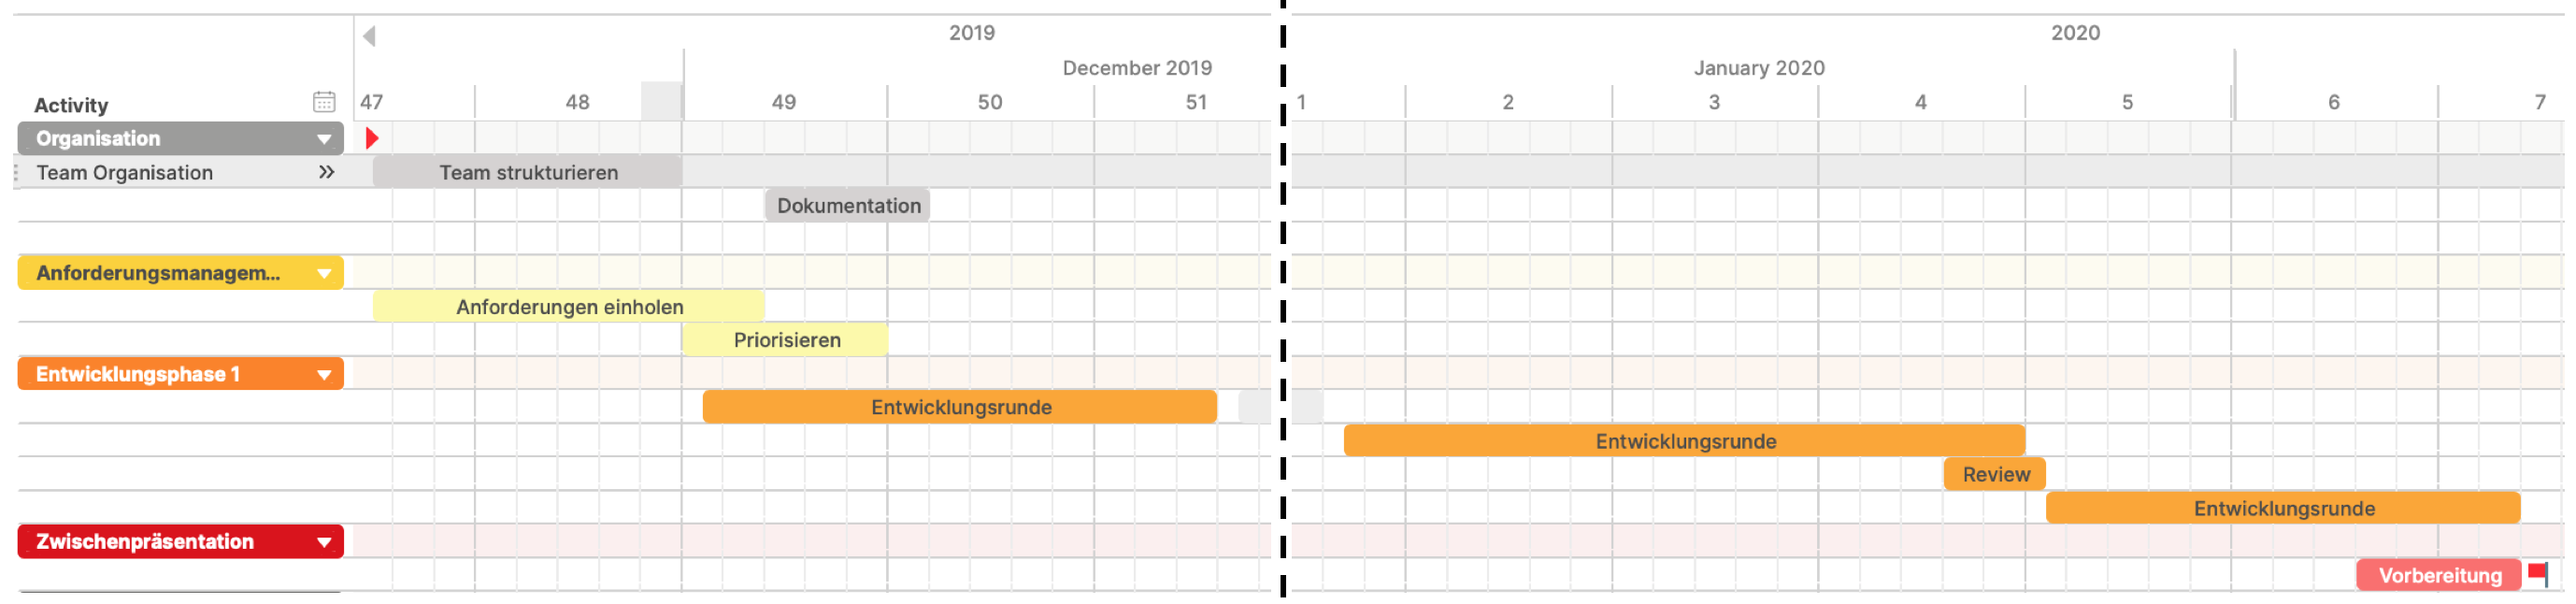
\includegraphics[width=\textwidth]{img/GanttSemester5.png}
	\captionsetup{format=hang}
	\caption[Grobe Übersicht Ganttdiagramm Semester 5]{\label{fig:Gantt5}Grobe Übersicht Ganttdiagramm Semester 5}
\end{figure}

In Abbildung \vref{fig:Gantt6}

\begin{figure}[H]
	\centering 
	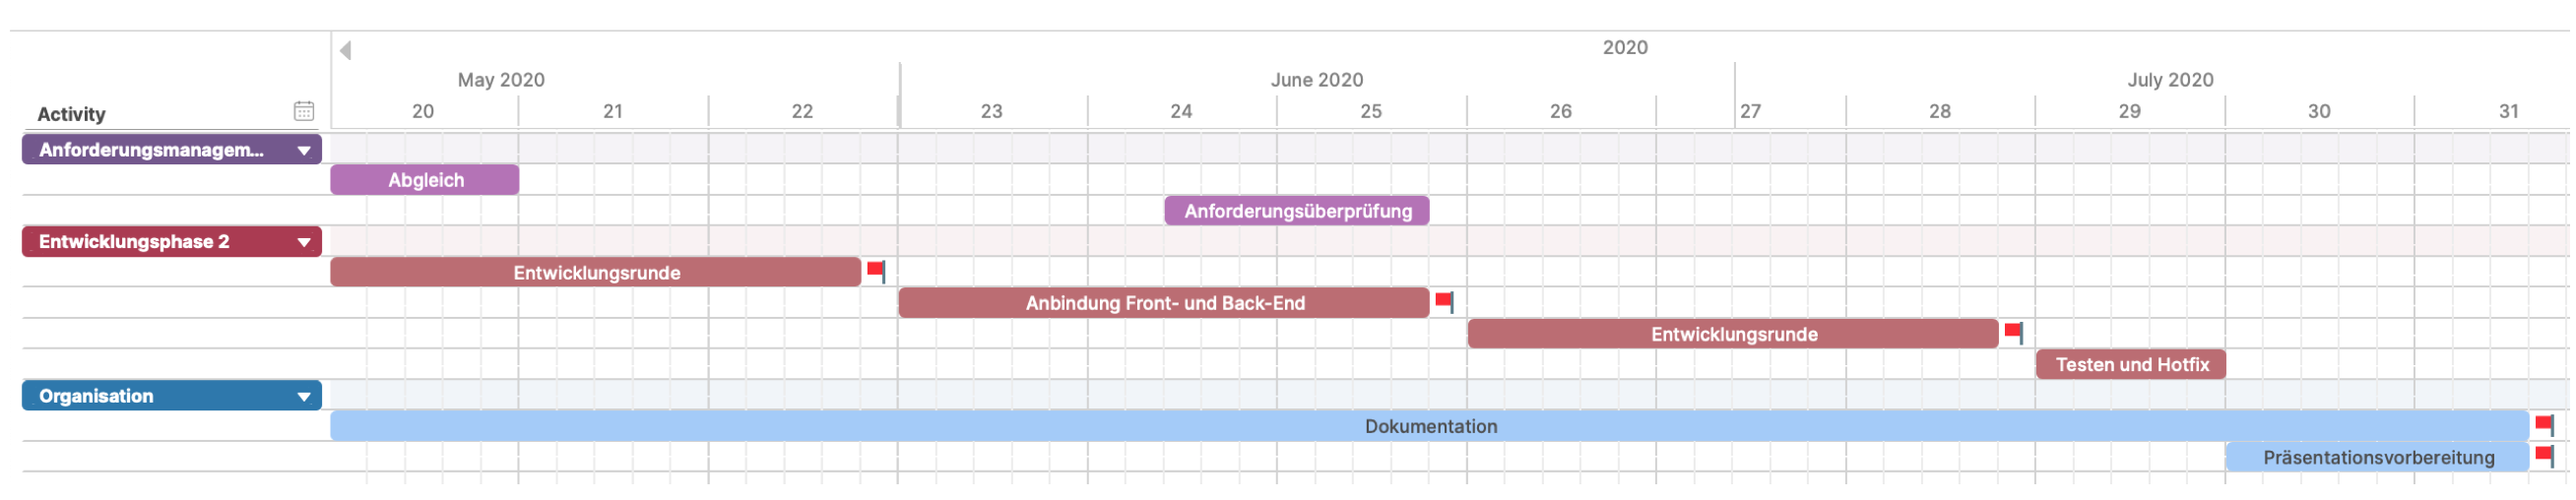
\includegraphics[width=\textwidth]{img/GanttSemester6.png}
	\captionsetup{format=hang}
	\caption[Grobe Übersicht Ganttdiagramm Semester 6]{\label{fig:Gantt6}Grobe Übersicht Ganttdiagramm Semester 6}
\end{figure}